\documentclass[conference]{IEEEtran}
% IEEE SmartGridComm: standard two-column IEEE conference format, up to six pages.
\usepackage[T1]{fontenc}
\usepackage{amsmath,amssymb,amsfonts,amsthm,bm}
\usepackage{graphicx}
\graphicspath{{figures/}}
\usepackage{booktabs,array,multirow}
\usepackage{xcolor}
\usepackage{enumitem}
\usepackage{cite}
\usepackage{url}
\usepackage{tikz}
\usetikzlibrary{arrows.meta,positioning,fit,calc,backgrounds}
\usepackage[hidelinks]{hyperref}

\newcommand{\method}{PRISM-XAI}
\newcommand{\mapxai}{MAP-XAI}
\newtheorem{proposition}{Proposition}
\newtheorem{corollary}{Corollary}
% Auto-generated by analysis/make_figures.py from the result files. Do not edit by hand.
\newcommand{\mapTrafficDiff}{36.40}
\newcommand{\mapTrafficCI}{3.32}
\newcommand{\mapTrafficRel}{15.72}
\newcommand{\mapPairs}{120}
\newcommand{\mapPrismKbit}{207.3}
\newcommand{\mapMapKbit}{243.7}
\newcommand{\mapRecallDiffPP}{-0.08}
\newcommand{\mapRecallQ}{0.53}
\newcommand{\mapCovDiffPP}{-0.01}
\newcommand{\mapTrafficQexp}{-41}
\newcommand{\mapExtRedMin}{82.0}
\newcommand{\mapExtRedMax}{94.8}
\newcommand{\paceOPSDEvUp}{48}
\newcommand{\paceOPSDEvDown}{0}
\newcommand{\paceOPSDEvN}{54}
\newcommand{\paceOPSDEvMed}{+12.3}
\newcommand{\paceOPSDEvCovO}{14.5}
\newcommand{\paceOPSDEvCovV}{31.6}
\newcommand{\paceOPSDEvAoxO}{182}
\newcommand{\paceOPSDEvAoxV}{44}
\newcommand{\paceOPSDEvKbit}{51.2}
\newcommand{\paceOPSDEvKbitRel}{15.1}
\newcommand{\paceOPSDEvEps}{0.65}
\newcommand{\paceOPSDEvRecUp}{28}
\newcommand{\paceOPSDPaUp}{40}
\newcommand{\paceOPSDPaDown}{0}
\newcommand{\paceOPSDPaN}{54}
\newcommand{\paceOPSDPaMed}{+6.5}
\newcommand{\paceOPSDPaCovO}{14.5}
\newcommand{\paceOPSDPaCovV}{25.5}
\newcommand{\paceOPSDPaAoxO}{182}
\newcommand{\paceOPSDPaAoxV}{45}
\newcommand{\paceOPSDPaKbit}{14.3}
\newcommand{\paceOPSDPaKbitRel}{4.2}
\newcommand{\paceOPSDPaEps}{0.93}
\newcommand{\paceOPSDPaRecUp}{9}
\newcommand{\paceUCIEvUp}{40}
\newcommand{\paceUCIEvDown}{5}
\newcommand{\paceUCIEvN}{54}
\newcommand{\paceUCIEvMed}{+5.1}
\newcommand{\paceUCIEvCovO}{12.7}
\newcommand{\paceUCIEvCovV}{20.9}
\newcommand{\paceUCIEvAoxO}{164}
\newcommand{\paceUCIEvAoxV}{44}
\newcommand{\paceUCIEvKbit}{86.5}
\newcommand{\paceUCIEvKbitRel}{8.5}
\newcommand{\paceUCIEvEps}{1.95}
\newcommand{\paceUCIEvRecUp}{23}
\newcommand{\paceUCIPaUp}{15}
\newcommand{\paceUCIPaDown}{6}
\newcommand{\paceUCIPaN}{54}
\newcommand{\paceUCIPaMed}{+1.2}
\newcommand{\paceUCIPaCovO}{12.7}
\newcommand{\paceUCIPaCovV}{16.1}
\newcommand{\paceUCIPaAoxO}{164}
\newcommand{\paceUCIPaAoxV}{45}
\newcommand{\paceUCIPaKbit}{45.3}
\newcommand{\paceUCIPaKbitRel}{5.1}
\newcommand{\paceUCIPaEps}{0.84}
\newcommand{\paceUCIPaRecUp}{8}
\newcommand{\paceNtests}{216}
\newcommand{\paceKbitUpMax}{1.9}
\newcommand{\paceKbitDownMax}{15.1}
\newcommand{\paceKbitMedOPSD}{-0.4}
\newcommand{\paceKbitMedUCI}{-3.0}
\newcommand{\paceEpsUpMax}{0.21}
\newcommand{\paceEpsDownMax}{1.95}
\newcommand{\heldRows}{7440}
\newcommand{\frEvOPSDAbove}{98.1}
\newcommand{\frEvOPSDMed}{+8.2}
\newcommand{\frEvOPSDN}{540}
\newcommand{\frOrOPSDAbove}{27.2}
\newcommand{\frOrOPSDMed}{-4.8}
\newcommand{\frOrOPSDN}{540}
\newcommand{\frPaOPSDAbove}{70.7}
\newcommand{\frPaOPSDMed}{+3.2}
\newcommand{\frPaOPSDN}{540}
\newcommand{\frOPSDKbitMax}{360}
\newcommand{\frEvUCIAbove}{100.0}
\newcommand{\frEvUCIMed}{+12.0}
\newcommand{\frEvUCIN}{540}
\newcommand{\frOrUCIAbove}{99.6}
\newcommand{\frOrUCIMed}{+7.1}
\newcommand{\frOrUCIN}{540}
\newcommand{\frPaUCIAbove}{100.0}
\newcommand{\frPaUCIMed}{+8.3}
\newcommand{\frPaUCIN}{540}
\newcommand{\frUCIKbitMax}{1324}
\newcommand{\frCellsPos}{106}
\newcommand{\frCells}{108}
\newcommand{\opAoxOPSDCov}{75}
\newcommand{\opRrOPSDCov}{75}
\newcommand{\opAoxOPSDKbit}{3988}
\newcommand{\opEvOPSDCovMax}{54}
\newcommand{\opEvOPSDKbitMax}{248}
\newcommand{\opEvOPSDKbitMin}{88}
\newcommand{\opAoxUCICov}{100}
\newcommand{\opRrUCICov}{100}
\newcommand{\opAoxUCIKbit}{5300}
\newcommand{\opEvUCICovMax}{43}
\newcommand{\opEvUCIKbitMax}{891}
\newcommand{\opEvUCIKbitMin}{311}
\newcommand{\claimTested}{52}
\newcommand{\claimSupported}{48}
\newcommand{\claimAll}{180}
\newcommand{\claimUntested}{128}
\newcommand{\claimDegenerateN}{24}
\newcommand{\claimDegenerateS}{24}
\newcommand{\claimWeakN}{24}
\newcommand{\claimWeakS}{20}
\newcommand{\claimStrongN}{4}
\newcommand{\claimStrongS}{4}
\newcommand{\diagBlKappaNNmin}{0.41}
\newcommand{\diagBlKappaNNmax}{0.53}
\newcommand{\diagBlKappaDPmax}{0.009}
\newcommand{\diagBlRatioMin}{188}
\newcommand{\diagBlRatioMax}{203}
\newcommand{\diagBlRatioNNmax}{1.12}
\newcommand{\diagUciRatioMin}{105}
\newcommand{\diagUciRatioMax}{134}
\newcommand{\diagUciKappaNNmax}{0.19}
\newcommand{\diagPrKappaNNmin}{-0.016}
\newcommand{\diagPrKappaNNmax}{0.032}
\newcommand{\diagSeeds}{11, 22, 33}
\newcommand{\diagRuns}{576}
\newcommand{\lockSha}{7af98e454aab}
\newcommand{\lockVtwoSha}{9005dfd6231f}
\newcommand{\redKappaOpsd}{-0.006}
\newcommand{\redKappaUci}{+0.026}
\newcommand{\redMech}{level12\_g0.1}
\newcommand{\redAbsMax}{0.026}
\newcommand{\redAllAbsMax}{0.028}
\newcommand{\redNconfigs}{8}
\newcommand{\propMaxRelErr}{4.1}
\newcommand{\propK}{400}
\newcommand{\propEFeight}{322}
\newcommand{\propLvEight}{1.30}
\newcommand{\sigPrismLo}{0.64}
\newcommand{\sigPrismHi}{3.98}
\newcommand{\sigBase}{8}

\makeatletter\newcommand{\rowsinput}[1]{\@@input #1 }\makeatother

\setlength{\textfloatsep}{6pt plus 2pt minus 2pt}
\setlength{\floatsep}{5pt plus 2pt minus 2pt}
\setlength{\dbltextfloatsep}{6pt plus 2pt minus 2pt}
\setlength{\abovecaptionskip}{3pt}

\begin{document}

\title{Private Explanation Streaming at the Smart-Grid Edge:\\
Budget Pacing Restores Timeliness, Error Feedback Erases Fidelity}

\author{
\IEEEauthorblockN{Nilab Sarwari, Poushali Sengupta, Sabita Maharjan}
\IEEEauthorblockA{Department of Informatics, University of Oslo, Norway\\
\{nilabs,poushali,sabita\}@ifi.uio.no}
}

\maketitle

\begin{abstract}
Grid operators increasingly want feature attributions that explain household
load forecasts, but streaming them from smart-meter endpoints costs uplink
capacity and differential-privacy (DP) budget. We study this problem with
\mapxai{}, a DP packetizer for attribution updates, and \method{}, an uplink
scheduler that uses only public state, and report three findings under a
pre-registered tune\,$\rightarrow$\,lock\,$\rightarrow$\,confirm protocol on two
public datasets. (i) At matched service and privacy, \method{} sends
\mapTrafficRel\% fewer bits than \mapxai{} alone over \mapPairs{} paired runs.
(ii) The original scheduler spends its privacy budget early and leaves endpoints
stale; a budget-pacing gate that changes neither the per-release noise nor the
budget raises critical-event coverage in \paceOPSDEvUp/\paceOPSDEvN{} (OPSD) and
\paceUCIEvUp/\paceUCIEvN{} (UCI) configurations on fresh seeds (Holm-corrected),
and, descriptively, places \method{} above the throttled-baseline traffic--coverage envelope in
\frEvOPSDAbove\% and \frEvUCIAbove\% of held-out runs. (iii) No evaluated method
recovers which feature group drives a critical event: Cohen's $\kappa\approx0$
throughout. We show why. Clipped error-feedback reconstruction lets DP noise
accumulate to a steady-state error of about $d\sigma^2\Delta^2/2C$; it matches the
simulator within \propMaxRelErr\% and explains the \diagBlRatioMin--\diagBlRatioMax$\times$ drift we measure.
A corollary gives the release count needed for fidelity, and a pre-registered
redesign confirms the limit. Timeliness is achievable under DP at these
budgets; fine-grained explanation fidelity is not.
\end{abstract}

\begin{IEEEkeywords}
smart-grid communications, differential privacy, explainable AI, uplink
scheduling, age of information, privacy budget pacing
\end{IEEEkeywords}

% =====================================================================
\section{Introduction}
% =====================================================================
Feature attributions such as SHAP~\cite{lundberg2017shap} tell an operator
\emph{why} a load forecast changed, and are studied for load forecasting and
grid monitoring~\cite{baur2024loadxai,gebhard2025anomaly}. When forecasts are
produced at household endpoints, their attributions must travel over a shared
uplink to the edge. Attributions leak information about household
behaviour~\cite{shokri2021privacy}, so each release should be protected with DP
and charged to a finite budget~\cite{dwork2006calibrating,mironov2017rdp}. The
operator therefore receives a \emph{stream of noisy, compressed, rate-limited}
explanations. Two questions decide whether such a stream is useful: does an
explanation arrive while it still matters (timeliness), and does it still say
what the true attribution says (fidelity)?

Prior work covers each ingredient separately. Federated and hierarchical XAI
expose privacy and communication costs of explanation
sharing~\cite{gholizade2026fedxai,sengupta2026hxai}. Age-of-information (AoI)
scheduling keeps status updates fresh under limited
opportunities~\cite{kaul2012aoi,yates2019aoi,aoi2025feedback}. Error feedback
makes compressed updates converge in distributed
learning~\cite{karimireddy2019ef}. DP training composes many noisy
releases~\cite{abadi2016dpsgd}. To our knowledge no work measures what happens
to timeliness and fidelity when the three meet on a smart-grid uplink.

We report one positive result for timeliness, one negative result for fidelity,
and a mechanism that explains the negative result.
\begin{itemize}[leftmargin=*]
\item \textbf{Scheduling under DP (Sec.~\ref{sec:system}).} \mapxai{} turns
attribution changes into clipped, Gaussian-perturbed, sparsified packets with
zCDP/RDP accounting. \method{} chooses endpoints and packet modes, or abstains,
from public state only. At matched coverage, recall and spent privacy it sends
\mapTrafficRel\% fewer bits than \mapxai{} alone.
\item \textbf{Budget pacing (Sec.~\ref{sec:pacing}).} We identify a
front-loading failure: the budget is exhausted early and endpoints stay stale. A
token-bucket pacing gate fixes it without touching the noise level or budget.
The fix is confirmed on fresh seeds with a lock written before any held-out run.
\item \textbf{A fidelity limit (Sec.~\ref{sec:theory}).} We prove that clipped
error-feedback reconstruction converges to a noise-dominated steady state, give
the release count any unbiased reconstruction needs, and confirm both on real
data, including a pre-registered redesign that does not cross the limit.
\item \textbf{Honest operating points (Sec.~\ref{sec:results}).} We separate
wins against strong, weak and non-functional baselines, and report where
\method{} sits on the traffic--coverage plane.
\end{itemize}

\begin{figure*}[t]
\centering
\resizebox{\textwidth}{!}{% Conceptual pipeline figure (full text width, drawn at 18 cm so scale is ~1).
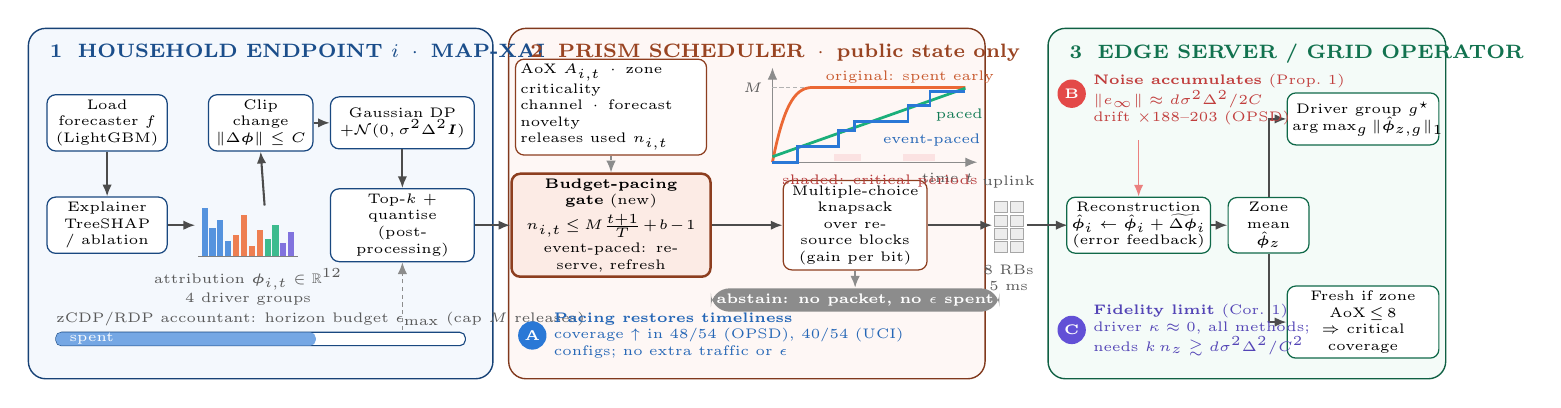
\begin{tikzpicture}[
  x=1cm, y=1cm,
  font=\tiny, >={Latex[length=1.5mm,width=1.2mm]},
  lane/.style={rounded corners=2.2mm, draw=#1!55!black, line width=0.5pt, fill=#1!5},
  lanetitle/.style={font=\bfseries\scriptsize, text=#1!65!black, anchor=north west},
  box/.style={rounded corners=1.1mm, draw=#1!60!black, fill=white, line width=0.45pt,
              align=center, inner sep=2.2pt, minimum height=7mm, text width=#1W},
  bx/.style={rounded corners=1.1mm, draw=#1!60!black, fill=white, line width=0.45pt,
             align=center, inner sep=1.8pt, minimum height=6.6mm, font=\tiny},
  pill/.style={rounded corners=2.4mm, fill=#1, text=white, font=\bfseries\tiny,
               inner sep=2pt},
  flow/.style={->, line width=0.75pt, draw=black!70},
  pub/.style={->, line width=0.5pt, draw=black!45, dash pattern=on 1.6pt off 1.2pt},
  note/.style={font=\tiny, text=black!65, align=center},
  badge/.style={circle, fill=#1, text=white, font=\bfseries\tiny, inner sep=0.5pt, minimum size=3.6mm},
  find/.style={font=\tiny, align=left, anchor=west, text=#1!85!black},
]
\definecolor{cblue}{HTML}{2A78D6}\definecolor{corange}{HTML}{EB6834}
\definecolor{caqua}{HTML}{1BAF7A}\definecolor{cviolet}{HTML}{6250D6}
\definecolor{cred}{HTML}{E34948}

% ---------------- lanes ----------------
\draw[lane=cblue]   (0,0)     rectangle (5.9,4.45);
\draw[lane=corange] (6.1,0)   rectangle (12.15,4.45);
\draw[lane=caqua]   (12.95,0) rectangle (18.0,4.45);
\node[lanetitle=cblue]   at (0.15,4.37) {1 \;HOUSEHOLD ENDPOINT $i$ \,$\cdot$\, MAP-XAI};
\node[lanetitle=corange] at (6.25,4.37) {2 \;PRISM SCHEDULER \,$\cdot$\, public state only};
\node[lanetitle=caqua]   at (13.1,4.37) {3 \;EDGE SERVER / GRID OPERATOR};

% ---------------- lane 1: endpoint ----------------
\node[bx=cblue, text width=14mm] (fc) at (1.0,3.25) {Load forecaster $f$\\(LightGBM)};
\node[bx=cblue, text width=14mm] (xp) at (1.0,1.95) {Explainer\\TreeSHAP / ablation};
\draw[flow] (fc) -- (xp);
\begin{scope}[shift={(2.2,1.55)}]
  \foreach \h [count=\k from 0] in {0.62,0.36,0.47,0.20}{\fill[cblue!80] (\k*0.1,0) rectangle ++(0.078,\h);}
  \foreach \h [count=\k from 4] in {0.28,0.53,0.14,0.34}{\fill[corange!85] (\k*0.1,0) rectangle ++(0.078,\h);}
  \foreach \h [count=\k from 8] in {0.22,0.40}{\fill[caqua!85] (\k*0.1,0) rectangle ++(0.078,\h);}
  \foreach \h [count=\k from 10] in {0.17,0.31}{\fill[cviolet!80] (\k*0.1,0) rectangle ++(0.078,\h);}
  \draw[black!50, line width=0.3pt] (-0.04,0) -- (1.22,0);
  \node[note, anchor=north] at (0.59,-0.03) {attribution $\bm\phi_{i,t}\in\mathbb R^{12}$\\4 driver groups};
\end{scope}
\draw[flow] (xp.east) -- (2.12,1.95);
\node[bx=cblue, text width=12mm] (clip) at (2.95,3.25) {Clip change\\$\|\Delta\bm\phi\|\le C$};
\node[bx=cblue, text width=17mm] (gau) at (4.75,3.25) {Gaussian DP\\$+\mathcal N(0,\sigma^2\Delta^2\bm I)$};
\node[bx=cblue, text width=17mm] (tk) at (4.75,1.95) {Top-$k$ + quantise\\(post-processing)};
\draw[flow] (3.0,2.2) -- (clip.south);
\draw[flow] (clip) -- (gau);
\draw[flow] (gau) -- (tk);
\begin{scope}[shift={(0.35,0.42)}]
  \node[note, anchor=south west, inner sep=0pt] at (0,0.24) {zCDP/RDP accountant: horizon budget $\epsilon_{\max}$ (cap $M$ releases)};
  \draw[rounded corners=0.7mm, draw=cblue!60!black, fill=white, line width=0.4pt] (0,0) rectangle (5.2,0.17);
  \fill[rounded corners=0.7mm, cblue!65] (0,0) rectangle (3.3,0.17);
  \node[note, text=white, anchor=west] at (0.05,0.085) {spent};
\end{scope}
\draw[pub] (4.75,0.62) -- (tk.south);

% ---------------- lane 2: scheduler ----------------
\node[bx=corange, text width=23mm, align=left] (state) at (7.4,3.45)
  {AoX $A_{i,t}$ \,$\cdot$\, zone criticality\\channel \,$\cdot$\, forecast novelty\\releases used $n_{i,t}$};
\node[bx=corange, text width=24mm, fill=corange!13, line width=0.9pt] (gate) at (7.4,1.95)
  {\textbf{Budget-pacing gate} (new)\\[1pt]$n_{i,t}\!\le\! M\frac{t+1}{T}\!+\!b\!-\!1$\\[1pt]event-paced: reserve, refresh};
\node[bx=corange, text width=17mm] (knap) at (10.5,1.95) {Multiple-choice knapsack\\over resource blocks\\(gain per bit)};
\draw[flow] (tk.east) -- (gate.west);
\draw[pub] (state) -- (gate);
\draw[flow] (gate) -- (knap);
\node[pill=black!45] (abst) at (10.5,1.0) {abstain: no packet, no $\epsilon$ spent};
\draw[flow, draw=black!45] (knap) -- (abst);
\begin{scope}[shift={(9.45,2.75), xscale=0.92, yscale=0.95}]
  \draw[black!45, line width=0.35pt, ->] (0,0) -- (2.6,0) node[note, anchor=north east, xshift=2pt, yshift=-0.5pt] {time $t$};
  \draw[black!45, line width=0.35pt, ->] (0,0) -- (0,1.2);
  \node[note, anchor=south east, rotate=90] at (-0.03,0) {};
  \draw[black!30, dash pattern=on 1.5pt off 1pt, line width=0.35pt] (0,0.95) -- (2.45,0.95);
  \node[note, anchor=east] at (0,0.95) {$M$};
  \fill[cred!16] (0.78,0.01) rectangle (1.12,0.11); \fill[cred!16] (1.66,0.01) rectangle (2.06,0.11);
  \draw[corange, line width=1pt] (0,0) .. controls (0.16,0.82) and (0.32,0.95) .. (0.52,0.95) -- (2.45,0.95);
  \draw[caqua, line width=1pt] (0,0.07) -- (2.45,0.94);
  \draw[cblue, line width=1pt] (0,0) -- (0.32,0) -- (0.32,0.2) -- (0.84,0.2) -- (0.84,0.4) -- (1.04,0.4) -- (1.04,0.52)
        -- (1.72,0.52) -- (1.72,0.72) -- (2.0,0.72) -- (2.0,0.9) -- (2.45,0.9);
  \node[note, text=corange!85!black, anchor=west] at (0.55,1.08) {original: spent early};
  \node[note, text=caqua!70!black, anchor=west] at (1.95,0.6) {paced};
  \node[note, text=cblue!85!black, anchor=west] at (1.28,0.28) {event-paced};
  \node[note, text=cred!80!black, anchor=north west] at (0.0,-0.04) {shaded: critical periods};
\end{scope}

% ---------------- uplink ----------------
\begin{scope}[shift={(12.27,1.6)}]
  \foreach \r in {0,...,3}{\foreach \c in {0,1}{\draw[black!35, fill=black!7, line width=0.3pt] (\c*0.2,\r*0.17) rectangle ++(0.17,0.14);}}
  \node[note, anchor=north] at (0.18,-0.03) {8 RBs\\5 ms};
  \node[note, anchor=south] at (0.18,0.7) {uplink};
\end{scope}
\draw[flow] (knap.east) -- (12.24,1.95);
\draw[flow] (12.68,1.95) -- (13.2,1.95);

% ---------------- lane 3: operator ----------------
\node[bx=caqua, text width=17mm] (recon) at (14.1,1.95)
  {Reconstruction\\$\hat{\bm\phi}_i\leftarrow\hat{\bm\phi}_i+\widetilde{\Delta\bm\phi}_i$\\(error feedback)};
\node[bx=caqua, text width=9mm] (zone) at (15.75,1.95) {Zone mean\\$\hat{\bm\phi}_z$};
\node[bx=caqua, text width=18mm] (drv) at (16.95,3.3) {Driver group $g^\star$\\$\arg\max_g\|\hat{\bm\phi}_{z,g}\|_1$};
\node[bx=caqua, text width=18mm] (fresh) at (16.95,0.72) {Fresh if zone AoX\,$\le$\,8\\$\Rightarrow$ critical coverage};
\draw[flow] (recon) -- (zone);
\draw[flow] (zone.north) |- (drv.west);
\draw[flow] (zone.south) |- (fresh.west);

% ---------------- findings ----------------
\node[badge=cblue] (b1) at (6.4,0.55) {A};
\node[find=cblue] at (6.55,0.55) {\textbf{Pacing restores timeliness}\\coverage $\uparrow$ in \paceOPSDEvUp/\paceOPSDEvN{} (OPSD), \paceUCIEvUp/\paceUCIEvN{} (UCI)\\configs; no extra traffic or $\epsilon$};
\node[badge=cred] (b2) at (13.25,3.62) {B};
\node[find=cred] at (13.4,3.55) {\textbf{Noise accumulates} (Prop.~1)\\$\|e_\infty\|\approx d\sigma^2\Delta^2/2C$\\drift $\times$\diagBlRatioMin--\diagBlRatioMax{} (OPSD)};
\draw[cred!70, line width=0.55pt, ->] (14.1,3.03) -- (recon.north);
\node[badge=cviolet] (b3) at (13.25,0.62) {C};
\node[find=cviolet] at (13.4,0.62) {\textbf{Fidelity limit} (Cor.~1)\\driver $\kappa\approx 0$, all methods;\\needs $k\,n_z\gtrsim d\sigma^2\Delta^2/C^2$};
\end{tikzpicture}
}
\caption{System and findings. \textbf{(1)} A trusted endpoint explains its load
forecast and releases the clipped attribution change through a Gaussian
mechanism (\mapxai{}). \textbf{(2)} \method{} admits packets through the new
budget-pacing gate and a multiple-choice knapsack, using only public state, or
abstains. Inset (schematic): the original scheduler spends its release cap early;
paced variants spread it over the horizon, and event-paced spends it during
critical periods. \textbf{(3)} The operator reconstructs by error feedback,
averages per zone, names the driver group, and counts a critical event as covered
if the zone is fresh. Badges summarise Sec.~\ref{sec:results}.}
\label{fig:concept}
\end{figure*}

% =====================================================================
\section{System Model}\label{sec:system}
% =====================================================================
\subsection{Endpoints, explanations and threat model}
Households $\mathcal H=\{1,\dots,N\}$ are grouped into zones $\mathcal H_z$ with
$n_z=|\mathcal H_z|$. At slot $t$ endpoint $i$ forecasts its load and computes an
attribution $\bm\phi_{i,t}\in\mathbb R^{d}$, $d=12$, over lag, rolling and
calendar features that form four fixed driver groups $\mathcal G$. The operator's
question at a critical zone-slot is the driver group
$g^\star_{z,t}=\arg\max_{g}\sum_{j\in g}|\bar\phi_{z,t,j}|$ of the zone-mean
attribution. Raw data and non-private attributions stay at the trusted endpoint.
The edge sees every transmitted packet. Content privacy is protected by DP;
timing side channels are outside the guarantee.

\subsection{\mapxai{}: private packets}
Let $\hat{\bm\phi}_{i}$ be the operator's current reconstruction, which is a
function of earlier releases only. The endpoint clips the change
$\Delta\bm\phi_{i,t}=\bm\phi_{i,t}-\hat{\bm\phi}_{i}$ to radius $C_i$ and releases
\begin{equation}
\widetilde{\Delta\bm\phi}_{i,t}=\mathrm{clip}_{C_i}(\Delta\bm\phi_{i,t})+\bm n_{i,t},\qquad
\bm n_{i,t}\sim\mathcal N(0,\sigma^2\Delta_i^2\bm I_d),\label{eq:gauss}
\end{equation}
with $\Delta_i=C_i$ under add/remove adjacency. Top-$k$ selection and
quantization follow as post-processing. A mode $m=(k,q,\sigma)$ costs
$S_0+k(\lceil\log_2 d\rceil+q+1)$ bits and $\rho=1/(2\sigma^2)$ zCDP per release,
composed additively and converted to $(\epsilon,\delta)$-DP~\cite{bun2016zcdp}. An
endpoint never exceeds $\epsilon_{\max}$. Privacy is charged on exposure, even if
the packet is later lost. On delivery the operator updates by error feedback,
$\hat{\bm\phi}_i\leftarrow\hat{\bm\phi}_i+\widetilde{\Delta\bm\phi}_{i,t}$.

\subsection{\method{}: public-state scheduling}
Each slot, \method{} scores the admissible modes of each endpoint by expected
explanation-loss reduction per bit. The score uses age of explanation (AoX)
$A_{i,t}$, forecast-derived zone criticality, channel state and forecast novelty,
never the private residual. It then solves a multiple-choice knapsack over
eight resource blocks under a 5\,ms deadline, in $O(NMB)$ time. Abstaining is
always feasible and spends no privacy. \method{} calibrates each release's noise
so that a cap of $M$ releases exactly exhausts $\epsilon_{\max}$; this gives
$\sigma\in[\sigPrismLo,\sigPrismHi]$ over our grid, against $\sigma=\sigBase$ for
the fixed-DP baselines.

% =====================================================================
\section{Budget Pacing}\label{sec:pacing}
% =====================================================================
A critical event is \emph{covered} when its zone's mean AoX is at most eight
slots. One delivery therefore keeps an endpoint useful for at most eight slots,
and coverage is bounded by how evenly the $M$ releases are spread. The original
\method{} admits a release whenever its public score is high. High scores cluster
early, so the cap is reached early and the endpoint stays silent for the rest of
the horizon (Fig.~\ref{fig:concept}, inset). On held-out runs the original
scheduler's mean AoX is \paceOPSDEvAoxO{} slots on OPSD over a 512-slot horizon.
This is a pacing failure, not a shortage of budget.

The \emph{pacing gate} admits endpoint $i$ at slot $t$ only if it holds a token,
\begin{equation}
\tau_{i,t}=M\,\tfrac{t+1}{T}+b-n_{i,t}\ \ge\ 1,\label{eq:token}
\end{equation}
where $n_{i,t}$ is the number of releases used and $b=1$. Unused tokens carry
over. The \emph{event-paced} variant adds two rules. A critical endpoint is
released only when its information is about to expire ($A_{i,t}\ge7$) or has never
been sent. A non-critical release must leave $R=2$ tokens in reserve for future
critical periods. Both rules read only the slot index, release counts, AoX and
the public criticality flag. Neither changes $\sigma$, $M$ or $\epsilon_{\max}$, so
the content-DP guarantee is unchanged.

% =====================================================================
\section{Why Fidelity Fails}\label{sec:theory}
% =====================================================================
Consider one endpoint with a fixed attribution $\bm\phi$ and reconstruction
error $\bm e_k=\hat{\bm\phi}^{(k)}-\bm\phi$ after $k$ deliveries. Write
$s=\sigma\Delta$ for the per-coordinate noise.

\begin{proposition}[Noise accumulation under clipped error feedback]\label{prop:ef}
If $\|\bm e_{k-1}\|\ge C$, then Eq.~\eqref{eq:gauss} with error-feedback update gives
$\mathbb E\big[\|\bm e_k\|^2\,\big|\,\bm e_{k-1}\big]=(\|\bm e_{k-1}\|-C)^2+d s^2.$
In the mean-field recursion $m_k^2=(m_{k-1}-C)^2+ds^2$, the RMS error converges
monotonically to
\begin{equation}
m^\star=\frac{d s^2+C^2}{2C}\;\approx\;\frac{d\,\sigma^2\Delta^2}{2C},\label{eq:steady}
\end{equation}
growing like $s\sqrt{dk}$ (a random walk) for about $k^\star\approx d s^2/(4C^2)$
releases.
\end{proposition}
\begin{proof}[Sketch]
When $\|\bm e\|\ge C$, clipping turns the correction into $-C\,\bm e/\|\bm e\|$,
so $\bm e_k=(1-C/\|\bm e_{k-1}\|)\bm e_{k-1}+\bm n_k$ with zero-mean independent
noise. Taking expectations gives the identity. The map
$m\mapsto\sqrt{(m-C)^2+ds^2}$ is a contraction above its unique fixed point
$m^\star$. Below the fixed point, $m_k^2-m_{k-1}^2\approx ds^2-2Cm_{k-1}$, which
gives the random-walk phase.
\end{proof}

The correction per release is at most $C$, while the injected noise has norm
about $s\sqrt d$. When $s\sqrt d\gg C$, later releases cannot cancel earlier noise.
For the baselines ($\sigma=\sigBase$, $\Delta=C$, $d=12$), Eq.~\eqref{eq:steady}
gives $m^\star\approx384C$, two orders of magnitude above any clipped
attribution. Fig.~\ref{fig:fidelity}(c) runs the simulator's own release function,
including Top-$k$ and quantization, for $\sigma\in\{2,8,12\}$. The recursion
matches it within \propMaxRelErr\% at $k=\propK$.

\begin{corollary}[Release count needed for fidelity]\label{cor:limit}
Let any unbiased estimator of a fixed clipped attribution ($\|\bm\phi\|\le C$) use
$k$ independent Gaussian releases per endpoint, and average over $n_z$
endpoints. Its zone-mean MSE is at least $ds^2/(k\,n_z)$ (Cram\'er--Rao
bound~\cite{kay1993}). Separating driver groups requires this noise to fall below
the signal, so
\begin{equation}
k\,n_z\ \gtrsim\ d\,\sigma^2\Delta^2/C^2 .\label{eq:limit}
\end{equation}
\end{corollary}
Releasing the level instead of the change and averaging the releases removes
the accumulation (Fig.~\ref{fig:fidelity}(c), dashed). Eq.~\eqref{eq:limit}
remains: at $\sigma=8$, OPSD ($n_z=3$) needs about 256 releases per endpoint of an
\emph{unchanged} attribution within one freshness window. At \method{}'s
$\sigma\le\sigPrismHi$ the requirement is smaller, but $M\le32$ releases over 512
slots leave each critical window with few fresh releases. The limit comes from
the per-release signal-to-noise ratio, not from the scheduler.

\begin{figure*}[t]
\centering
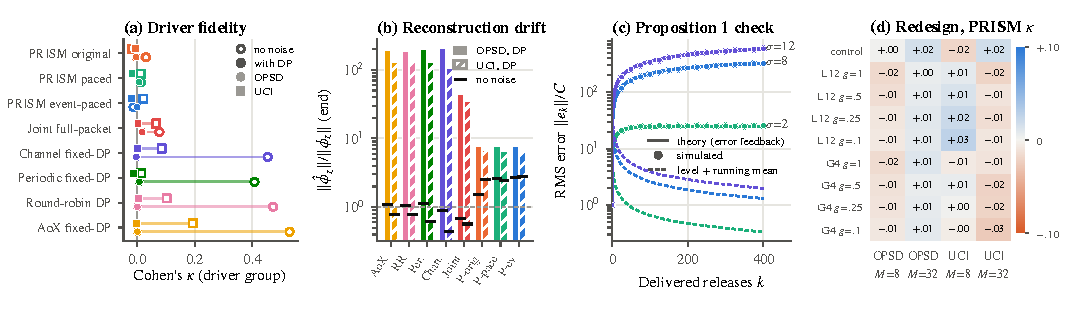
\includegraphics[width=\textwidth]{fig_fidelity.pdf}
\caption{Why fidelity fails (tuning seeds; diagnostic). \textbf{(a)} Driver
$\kappa$ with the same schedule run without noise (hollow) and with DP (filled).
\textbf{(b)} Reconstruction drift at the end of the horizon; bars with DP,
dashes without noise. \textbf{(c)} Prop.~\ref{prop:ef}: theory (lines) against
the simulator's release function (dots), and level release with running mean
(dashed). \textbf{(d)} Pre-registered redesign for event-paced \method{}: no
setup reaches the GO thresholds ($\kappa\ge0.10$ OPSD, $\ge0.05$ UCI).}
\label{fig:fidelity}
\end{figure*}

% =====================================================================
\section{Evaluation Protocol}\label{sec:protocol}
% =====================================================================
\textbf{Data and model.} We use OPSD household data (nine eligible households,
three zones) and UCI ElectricityLoadDiagrams20112014 (32 clients, four
zones)~\cite{opsd2020household,uci2015eld}. A LightGBM forecaster is explained
with TreeSHAP and with feature ablation. Each run has 96 calibration and 512
evaluation slots, with $\epsilon_{\max}\in\{8,16,32\}$ and $\delta=10^{-5}$. The
uplink trace follows 3GPP TR~38.901 path loss, shadowing, fading and bursty
failures~\cite{3gpp38901}. It is a scheduler-level stress trace, not a link-level
validation.

\textbf{Metrics.} \emph{Coverage}: fraction of critical zone-slots that are
fresh (zone AoX$\,\le8$ and quality certificate $\ge0.1$). \emph{Driver
fidelity}: Cohen's $\kappa$~\cite{cohen1960} between true and reconstructed
driver groups on all critical zone-slots. We use $\kappa$ because always guessing
the dominant group already agrees 95\% of the time on OPSD. We also report
traffic, spent $\epsilon$ and reconstruction drift
$\|\hat{\bm\phi}_z\|/\|\bm\phi_z\|$.

\textbf{Baselines.} Periodic, round-robin, channel-aware and AoX-aware fixed-DP
schedulers and joint full-packet scheduling. To trace their traffic--coverage
curves we throttle each with a deterministic duty cycle in $\{1,\dots,2^{-6}\}$;
these are throttled variants, not the published methods.

\textbf{Pre-registration.} Configurations ($M\in\{8,16,32\}$, score threshold
$\in\{1,3,5\}$, baseline duty) were chosen from ten tuning seeds only and locked
(SHA-256 \texttt{\lockVtwoSha\ldots}) before held-out runs. An earlier held-out
set was inspected, so all confirmatory numbers below use \emph{fresh} seeds
2001--2010 ($\heldRows$ runs). Seeds are the independent units: one paired test
per configuration, with Holm correction~\cite{holm1979}. Diagnostics and the
redesign use tuning seeds \diagSeeds{} only. The redesign's GO/NO-GO rule was
fixed in code and its decision locked (SHA-256 \texttt{\lockSha\ldots}).

% =====================================================================
\section{Results}\label{sec:results}
% =====================================================================
\subsection{Scheduling at matched service}
Table~\ref{tab:main} shows the 720-run matrix. \mapxai{} alone sends
\mapExtRedMin--\mapExtRedMax\% fewer bits than the external baselines, but at
much lower coverage, so these are different operating points, not wins. The
clean comparison is \method{} against \mapxai{}-only. The two meet the
matched-service rule (coverage and recall within 0.02, spent $\epsilon$ within
5\%) in all twelve conditions. \method{} saves
$\mapTrafficDiff\pm\mapTrafficCI$\,kbit per run (95\% CI, $n=\mapPairs$,
$q<10^{\mapTrafficQexp}$), a \mapTrafficRel\% reduction. Coverage changes by
$\mapCovDiffPP$ and recall by $\mapRecallDiffPP$ percentage points; neither is
detected.

\begin{table}[t]
\caption{Operating points in the 720-run matrix (means over 120 runs per row). Recall counts covered events whose driver group matches; with $\kappa\approx0$ (Sec.~\ref{sec:results}-D) it tracks coverage.}
\label{tab:main}
\centering\scriptsize\setlength{\tabcolsep}{3.4pt}
\begin{tabular}{lrrrr}
\toprule
Method & Traffic (kbit) & Coverage & Recall & $\epsilon^{\max}_{\rm spent}$\\
\midrule
\rowsinput{table_main_rows.tex}
\bottomrule
\end{tabular}
\end{table}

\subsection{Budget pacing restores timeliness}
Fig.~\ref{fig:pacing} plots every locked configuration on fresh seeds.
Event-paced coverage is significantly higher than the original's in
\paceOPSDEvUp/\paceOPSDEvN{} OPSD and \paceUCIEvUp/\paceUCIEvN{} UCI
configurations, and lower in none on OPSD and \paceUCIEvDown{} on UCI. The median
gains are $\paceOPSDEvMed$ and $\paceUCIEvMed$ percentage points. Mean coverage rises
from \paceOPSDEvCovO\% to \paceOPSDEvCovV\% (OPSD) and from \paceUCIEvCovO\% to
\paceUCIEvCovV\% (UCI). Mean AoX falls from \paceOPSDEvAoxO{} to
\paceOPSDEvAoxV{} slots on OPSD. Traffic changes by between $-\paceKbitDownMax$\% and
$+\paceKbitUpMax$\% (median $\paceKbitMedOPSD$\% OPSD, $\paceKbitMedUCI$\% UCI). The
maximum spent $\epsilon$ rises by at most \paceEpsUpMax{} and otherwise falls, by up
to \paceEpsDownMax. The gain therefore comes from \emph{when} the budget is spent,
not from spending more. Plain
pacing helps less (\paceOPSDPaUp{} and \paceUCIPaUp{} configurations), which shows
that aligning releases with critical periods matters.

\begin{figure}[t]
\centering
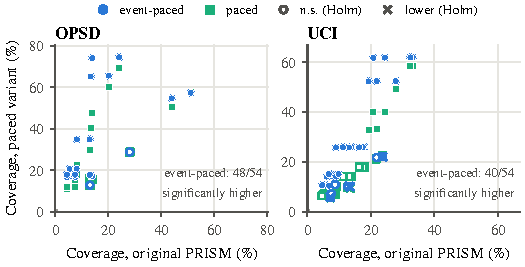
\includegraphics[width=\columnwidth]{fig_pacing.pdf}
\caption{Budget pacing on fresh seeds: each point is one locked configuration
(dataset$\times$XAI$\times\epsilon_{\max}\times M\times$threshold; 10 seeds each).
Points above the diagonal improve on the original scheduler. Filled markers:
Holm-significant increase; hollow: not significant; crosses: significant
decrease.}
\label{fig:pacing}
\end{figure}

\begin{figure}[t]
\centering
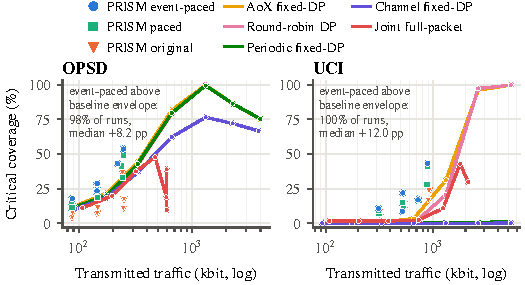
\includegraphics[width=\columnwidth]{fig_frontier.pdf}
\caption{Traffic--coverage operating points on fresh seeds. Lines trace each
throttled baseline over its duty cycles; markers are \method{} configurations.
The envelope is the best baseline coverage achievable at no more traffic, in the
same dataset, XAI method, $\epsilon_{\max}$ and seed. Descriptive; not part of
the locked hypotheses.}
\label{fig:frontier}
\end{figure}

\subsection{Where \method{} sits against baselines}
Fig.~\ref{fig:frontier} shows the full operating curves. At low traffic,
event-paced \method{} lies above the best baseline curve in
\frEvOPSDAbove\% (OPSD) and \frEvUCIAbove\% (UCI) of paired runs, with median
margins of $\frEvOPSDMed$ and $\frEvUCIMed$ percentage points. On OPSD, pacing is
what moves it there: the original scheduler is above the envelope in only
\frOrOPSDAbove\% of runs (median $\frOrOPSDMed$ points). At high traffic the
AoX-aware and round-robin baselines reach 75--100\% coverage, which \method{},
capped at $M\le32$ private releases, does not attempt. The locked matched-service
test reflects this (Table~\ref{tab:tier}). Traffic claims hold in
\claimSupported/\claimTested{} comparisons that had a tuning match, but
\claimDegenerateN{} of these are against baselines that are non-functional in
this setup ($<$5\% coverage). Only \claimStrongN{} are against a strong
baseline, and \claimUntested{} comparisons, including every one against the
AoX-aware and round-robin schedulers, had no match and were not tested.

\begin{table}[t]
\caption{Locked traffic claims on fresh seeds by strength of the matched
baseline (its coverage).}
\label{tab:tier}
\centering\scriptsize\setlength{\tabcolsep}{4pt}
\begin{tabular}{llrrr}
\toprule
Data & Baseline tier & Supported & Traffic red.\ (\%) & Base cov.\ (\%)\\
\midrule
\rowsinput{table_tier_rows.tex}
\bottomrule
\end{tabular}
\end{table}



\subsection{Driver fidelity: diagnosis}
On fresh seeds, every scheduler, baseline or \method{}, has driver
$\kappa\approx0$. Fig.~\ref{fig:fidelity} shows why. Run without noise on the
same schedule, the high-rate baselines identify the driver group on OPSD
($\kappa=\diagBlKappaNNmin$--$\diagBlKappaNNmax$). With DP, their $\kappa$ falls to
$|\kappa|\le\diagBlKappaDPmax$ and their reconstructions drift to
\diagBlRatioMin--\diagBlRatioMax$\times$ the true norm (UCI:
\diagUciRatioMin--\diagUciRatioMax$\times$), against about $1\times$ without noise.
This is the accumulation predicted by Prop.~\ref{prop:ef}. \method{}'s leaky
residual buffer avoids most of the drift ($\approx7\times$), but at $M\le32$ its
reconstruction is stale even without noise ($\kappa\in[\diagPrKappaNNmin,
\diagPrKappaNNmax]$). A pre-registered redesign then tested
\redNconfigs{} variants on tuning seeds. Each sent the level, either all 12
values or the four group magnitudes, with a running-mean update; noise level,
privacy charge and packet sizes were unchanged. The best setup
(\texttt{\redMech}) reached $\kappa=\redKappaOpsd$ on OPSD and $\redKappaUci$ on
UCI, far below the GO thresholds, so we did not spend the fresh confirmation
seeds. This matches Cor.~\ref{cor:limit}: removing the accumulation is necessary
but not sufficient.

% =====================================================================
\section{Discussion and Limitations}\label{sec:discussion}
% =====================================================================
\textbf{Design implications.} (i) Pace the DP budget against the freshness
window. It is free in privacy and moved \method{} above the baseline curve at
low traffic. (ii) Do not reconstruct DP-protected streams by clipped error
feedback when $\sigma\sqrt d\gg1$. Eq.~\eqref{eq:steady} predicts the resulting
noise floor. (iii) Fine-grained explanation fidelity needs
$k\,n_z\gtrsim d\sigma^2\Delta^2/C^2$. Fewer released dimensions,
zone-level aggregation before noise (e.g., secure
aggregation~\cite{bonawitz2017secagg}) or larger budgets are the levers; better
scheduling alone is not.

Table~\ref{tab:claims} lists what the paper does and does not claim.

\textbf{Limitations.} The uplink is simulated, and coverage is a freshness
proxy, not an operator outcome. Driver fidelity is measured against the
explainer's own attribution, not ground truth. The baselines are throttled
variants. The frontier analysis (Fig.~\ref{fig:frontier}) was not
pre-registered. Diagnostics use three tuning seeds. The DP guarantee covers
packet contents under add/remove adjacency, not transmission timing.


\begin{table}[t]
\caption{Claim--evidence map.}
\label{tab:claims}
\centering\scriptsize\setlength{\tabcolsep}{2.6pt}
\begin{tabular}{>{\raggedright\arraybackslash}p{0.27\columnwidth}>{\raggedright\arraybackslash}p{0.42\columnwidth}>{\raggedright\arraybackslash}p{0.22\columnwidth}}
\toprule
Claim & Evidence & Status\\
\midrule
\method{} saves traffic vs.\ \mapxai{} & $-\mapTrafficRel$\%, $n=\mapPairs$ paired runs, matched service & Supported\\
Pacing raises coverage & \paceOPSDEvUp/\paceOPSDEvN{} and \paceUCIEvUp/\paceUCIEvN{} configs, fresh seeds, Holm & Confirmatory\\
Above baseline envelope at low traffic & \frEvOPSDAbove\% and \frEvUCIAbove\% of held-out runs & Descriptive\\
Saves traffic vs.\ strong baselines & \claimStrongS/\claimStrongN{} tested; AoX and round-robin untested & Not claimed\\
Error feedback accumulates DP noise & Prop.~\ref{prop:ef}; drift \diagBlRatioMin--\diagBlRatioMax$\times$ & Supported\\
Driver-level explanation fidelity & $\kappa\approx0$ for all methods; redesign NO-GO & Not achieved\\
\bottomrule
\end{tabular}
\end{table}

\section{Conclusion}
Streaming differentially private explanations from smart-grid endpoints works
for \emph{timeliness}. Public-state scheduling cuts traffic by
\mapTrafficRel\% at matched service, and budget pacing raises critical-event
coverage at unchanged privacy and traffic. It does not work for
\emph{fidelity} at $\epsilon_{\max}\le32$. Clipped error feedback lets DP noise
accumulate to $d\sigma^2\Delta^2/2C$, and even an accumulation-free redesign
falls short of the release count in Cor.~\ref{cor:limit}. Code, locks and all
result files are released for reproduction.\footnote{Repository:
\url{https://github.com/Poushali96/PRISMXAI2026}. Generative AI tools assisted with
editing and code; the authors verified all results.}

\begin{thebibliography}{00}\footnotesize
\bibitem{lundberg2017shap} S.~M. Lundberg and S.-I. Lee, ``A unified approach to interpreting model predictions,'' in \emph{Proc. NeurIPS}, 2017, pp. 4765--4774.
\bibitem{baur2024loadxai} L.~Baur \emph{et al.}, ``Explainability and interpretability in electric load forecasting using machine learning techniques---A review,'' \emph{Energy and AI}, vol.~16, Art.~100358, 2024.
\bibitem{gebhard2025anomaly} T.~Gebhard, A.~Tundis, and F.~Steinke, ``Explainable anomaly detection for grid monitoring using probabilistic load forecasting,'' in \emph{Proc. IEEE SmartGridComm}, 2025.
\bibitem{shokri2021privacy} R.~Shokri, M.~Strobel, and Y.~Zick, ``On the privacy risks of model explanations,'' in \emph{Proc. AAAI/ACM AIES}, 2021, pp. 231--241.
\bibitem{dwork2006calibrating} C.~Dwork, F.~McSherry, K.~Nissim, and A.~Smith, ``Calibrating noise to sensitivity in private data analysis,'' in \emph{Proc. TCC}, 2006, pp. 265--284.
\bibitem{mironov2017rdp} I.~Mironov, ``R\'enyi differential privacy,'' in \emph{Proc. IEEE CSF}, 2017, pp. 263--275.
\bibitem{bun2016zcdp} M.~Bun and T.~Steinke, ``Concentrated differential privacy: Simplifications, extensions, and lower bounds,'' in \emph{Proc. TCC}, 2016, pp. 635--658.
\bibitem{gholizade2026fedxai} M.~Gholizade, F.~Ruffini, P.~Ducange, and F.~Marcelloni, ``Federated explainable artificial intelligence: Roles, architectures, evaluation, and open challenges,'' \emph{Expert Syst. Appl.}, vol.~331, Art.~133183, 2026.
\bibitem{sengupta2026hxai} P.~Sengupta, S.~Maharjan, F.~Eliassen, and Y.~Zhang, ``HXAI: Hierarchical privacy-preserving explainable AI in distributed energy systems,'' arXiv:2610.02504, 2026.
\bibitem{kaul2012aoi} S.~Kaul, R.~Yates, and M.~Gruteser, ``Real-time status: How often should one update?'' in \emph{Proc. IEEE INFOCOM}, 2012, pp. 2731--2735.
\bibitem{yates2019aoi} R.~D. Yates \emph{et al.}, ``Age of information: An introduction and survey,'' \emph{IEEE J. Sel. Areas Commun.}, vol.~39, no.~5, pp. 1183--1210, 2021.
\bibitem{aoi2025feedback} A.~Munari and L.~Badia, ``What's my age of information again? The role of feedback in AoI optimization under limited transmission opportunities,'' \emph{IEEE Trans. Commun.}, vol.~73, no.~11, pp. 10495--10508, 2025.
\bibitem{karimireddy2019ef} S.~P. Karimireddy, Q.~Rebjock, S.~U. Stich, and M.~Jaggi, ``Error feedback fixes SignSGD and other gradient compression schemes,'' in \emph{Proc. ICML}, 2019, pp. 3252--3261.
\bibitem{abadi2016dpsgd} M.~Abadi \emph{et al.}, ``Deep learning with differential privacy,'' in \emph{Proc. ACM CCS}, 2016, pp. 308--318.
\bibitem{kay1993} S.~M. Kay, \emph{Fundamentals of Statistical Signal Processing: Estimation Theory}. Prentice Hall, 1993.
\bibitem{opsd2020household} Open Power System Data, ``Household data,'' version 2020-04-15, 2020.
\bibitem{uci2015eld} A.~Trindade, ``ElectricityLoadDiagrams20112014,'' UCI Machine Learning Repository, 2015, doi: 10.24432/C58C86.
\bibitem{3gpp38901} 3GPP, ``Study on channel model for frequencies from 0.5 to 100 GHz,'' TR 38.901, Rel.~18.
\bibitem{cohen1960} J.~Cohen, ``A coefficient of agreement for nominal scales,'' \emph{Educ. Psychol. Meas.}, vol.~20, no.~1, pp. 37--46, 1960.
\bibitem{holm1979} S.~Holm, ``A simple sequentially rejective multiple test procedure,'' \emph{Scand. J. Statist.}, vol.~6, no.~2, pp. 65--70, 1979.
\bibitem{bonawitz2017secagg} K.~Bonawitz \emph{et al.}, ``Practical secure aggregation for privacy-preserving machine learning,'' in \emph{Proc. ACM CCS}, 2017, pp. 1175--1191.
\end{thebibliography}
\end{document}
